\documentclass[preprint,10pt]{elsarticle}
\setlength{\parindent}{0pt}
\usepackage[hscale=0.8, vscale=0.8]{geometry}

\usepackage{graphicx}
\usepackage{tikz}
\usepackage{verbatim}
\usepackage{subcaption} % for subfigures


% for algorithmicx package
\usepackage{algorithm}
\usepackage{algpseudocode}

% math stuff
\usepackage{mathpartir}
\usepackage{amssymb}
\usepackage{amsmath,amsthm}
\usepackage{pfsteps}
\usepackage{listings}
\usepackage{hyperref}

% my personal shortcuts
\usepackage{shortcuts}

% theorem and proof environments
\newtheorem{theorem}{Theorem}
\newtheorem{definition}{Definition}
\newtheorem{lemma}{Lemma}
\newtheorem{proposition}{Proposition}
\newtheorem{claim}{Proposition}
\newtheorem{example}{Example}
\newtheorem{corollary}{Corollary}
\newtheorem{fact}{Fact}[section]

%%% stuff borrowed from scribe.tex
\newcounter{lecnum}
\renewcommand{\thepage}{\thelecnum-\arabic{page}}
\renewcommand{\thesection}{\thelecnum.\arabic{section}}
\renewcommand{\theequation}{\thelecnum.\arabic{equation}}
\renewcommand{\thefigure}{\thelecnum.\arabic{figure}}
\renewcommand{\thetable}{\thelecnum.\arabic{table}}

%
% The following macro is used to generate the header.
%
%\newcommand{\lecture}[4]{
%   \pagestyle{myheadings}
%   \thispagestyle{plain}
%   \newpage
%   \setcounter{lecnum}{#1}
%   \setcounter{page}{1}
%   \noindent
%   \begin{center}
%   \framebox{
%      \vbox{\vspace{2mm}
%    \hbox to 6.28in { {\bf CS 421 Algorithms
%                        \hfill Winter 2014} }
%       \vspace{4mm}
%       \hbox to 6.28in { {\Large \hfill Homework #1: #2  \hfill} }
%       \vspace{2mm}
%       \hbox to 6.28in { {\it Prof: #3 \hfill Solutions By: #4} }
%      \vspace{2mm}}
%   }
%   \end{center}
%   \markboth{Lecture #1: #2}{Lecture #1: #2}
%   {\bf Note}: {\it the solution for problem 5 is due to Kleinberg; any copy/paste errors may be mine though :)
%   }
%   \vspace*{4mm}
%}


%\title {\bf CSE 421 -- Algorithms\\
%Winter 14\\
%Problem Set 3 Solutions}

%%% END OF STUFF USED FOR ALGORITHMS CLASS

\journal{idk}
\begin{document}

%\maketitle
%\lecture{4}{\today}{James Lee}{Armando Diaz Tolentino}

\begin{frontmatter}

%% Title, authors and addresses

%% use the tnoteref command within \title for footnotes;
%% use the tnotetext command for theassociated footnote;
%% use the fnref command within \author or \address for footnotes;
%% use the fntext command for theassociated footnote;
%% use the corref command within \author for corresponding author footnotes;
%% use the cortext command for theassociated footnote;
%% use the ead command for the email address,
%% and the form \ead[url] for the home page:
%% \title{Title\tnoteref{label1}}
%% \tnotetext[label1]{}
%% \author{Name\corref{cor1}\fnref{label2}}
%% \ead{email address}
%% \ead[url]{home page}
%% \fntext[label2]{}
%% \cortext[cor1]{}
%% \address{Address\fnref{label3}}
%% \fntext[label3]{}

\title{Our Super-Special Awesome Research Paper}

%% use optional labels to link authors explicitly to addresses:
%% \author[label1,label2]{}
%% \address[label1]{}
%% \address[label2]{}

\author{Armando Diaz and Siva Ramamoorthy}

\address{\{ ajdt, sivanr\}@cs.washington.edu}

\begin{abstract}
The Arbitrary Patter Formation(APF) problem requires a group of $n$  mobile robots form a  target pattern on 
the $\RR^2$ plane in finite time without explicit communication. 
APF has been studied in the literature under various
assumptions such as restrictions on target patterns, assumptions on the coordinate 
axes of each robot. All prior work has been in a deterministic setting. 
Here, we study APF when given access to randomness.
We revisit some of the established work, in particular an impossibility result for APF 
when $n$ is even and a OneAxis agreement exists between robots, and we apply randomness to break the impossibility result. 
\end{abstract}

\begin{keyword}
fat robots, abstract pattern formation, mobile robots
\end{keyword}

\end{frontmatter}

\section{Introduction}
% include sources that corroborate these uses 
A recent trend in robotics has been toward the development of simple, commodity robots that can
be composed and arranged in a number of configurations to perform a complex task. The benefits of using composable,
simple robots in lieu of monolithic single purpose robots include a greater ability to leverage prior work in
robotics, and greater localization of failures -- so that a single incapacitated robot in a group is replaced
and taken offline rather than an entire monolithic machine. In many settings, failure may be frequent due to 
hazardous conditions, and so priority is placed on making the mobile robots cost-effective and therefore 
as simple as possible. As such, communication between robots is either limited or not feasible. This presents a
new challenge in that a group of robots must cooperate to form a configuration without any explicit communication. \\

The Arbitrary Pattern Formation (APF) problem rises out of this challenge. Concretely, we are given
a set of $n$ robots. The position of each robot $i$ on the 2D plane is given by $p_i \in \RR^2$, and we
describe a configuration of robots $\EE$ as an $n$-tuple of positions $\EE = (x_1, \ldots x_n)$.
The APF problem requires the robots to form some arbitrary pattern $\PP = (p_1, \ldots p_n)$ in finite
time beginning from some initial configuration $\EE$. Furthermore, no pair of robots $i$, $j$ can 
communicate explicitly with each other. Each robot runs a local instance of some algorithm to
achieve consensus and can only perform three operations: \textit{Look, Move, and Wait}. A \textit{Look}
operation is an observation of the configuration $\EE_i$ of the other robots with respect to robot
$i$'s local view. A \textit{Move} operation is a straight line motion to a target point $t \in \RR^2$.
During a \textit{Wait} operation, a robot simply decides to remain at its current location. \\

In the following subsection we discuss in greater detail the various modelling choices that have been
considered in the literature; focusing on the modelling choices relevant to our contribution. In
section \ref{prevWork}, we give an incomplete account on results and recent work on the APF problem. We
emphasize results that our contribution depends upon or extends. In section \ref{ourRes}, we discuss
two distinct approaches we develop to solve the APF problem for any number of robots. Finally,
we conclude with \ref{conc} by discussing open problems, and unresolved questions in regard to our contribution.

\subsection{Robot Models} 
\label{models}
Due to the range of settings APF may be applied, a number of robot models have been considered 
in the literature. History oblivious models, for example, have insufficient memory to remember
a configuration $\EE$ that occurred in a previous Look-Move-Wait cycle. Robot vision is another 
source of modelling choice. Robots can be modelled to see arbitrarily far, up to some distance $\delta$, or
with some error in measurement $\epsilon$. Likewise, robots may be able to see through each other as in the 
\textit{transparent} model, or their line of sight may be limited by other robots as in the \textit{opaque}
model. \\

Two assumptions are particularly germane to the work we present in this paper. Many of the results in 
the literature, have been established for robots modelled as points on the 2D plane. Alternatively,
robots could be modelled as unit disks. The disk model is closer to the applied setting, and is being
% TODO: insert citation for gathering problem
studied more extensively in recent works. Another important assumption is that of compass orientations.
All robot models assume each robot $i$ possesses a \textit{compass} $C_i$ used to map an $x-y$ coordinate system
onto the 2D plane that it observes. In the most general case, each compass $C_i$ is arbitrarily oriented with
respect to the other robots' compasses. Thus, any two robots $i$ and $j$ may have very distinct notions
of the orientation of the $x$ and $y$ axes. Some models make a very strong assumption that all compasses $C_i$ 
are in complete agreement on the orientation of both axes. This assumption is referred to in the 
literature as \textit{consistent compass}. A weaker assumption, \textit{OneAxis} is 
that all robots' compasses agree on the orientation of just a single axis. \\% TODO: insert figure here

In our work, we examine a robot model that is history oblivious, disk-based, and (for one result) assumes OneAxis.
% synch vs async??


\section{Known results}
	\label{prevWork}
	We refer interested readers to \cite{flocchini12distrib} for a comprehensive survey of results for
	APF and related problems. In this section, we are primarily concerned with results directly relevant
	to our work. \\

	In \ref{models}, we introduced the consistent compass assumption. It is well-known that consistent compass 
	trivializes APF problem. 
	\begin{theorem} 
		With a consistent compass assumption, Arbitrary Pattern Formation is solvable, even in an asynchronous setting.
		\cite{flocchini08arbitrary}
	\end{theorem} 
	\begin{proof}
		The consistent compass assumption requires that all robots agree on the orientation of both compass
		axes. Since each robot knows the target pattern \textit{a priori}, each robot can independently compute
		a total ordering of the points constituting the pattern as shown in \ref{ccfig1}. In the example figure,
		the points are ordered by decreasing $y$-coordinate and then increasing $x$-coordinate. Likewise, 
		all of the robots can assign an ordering to themselves in a similar fashion as shown in \ref{ccfig2}.
		Having achieved this ordering, each robot is assigned to a unique position in the pattern, and the robots
		can move in order, one at a time to form the target pattern.
	\end{proof}
	
	\begin{figure}[H]
		\begin{subfigure}{0.5\textwidth}
		\label{ccfig1}
		\centering
		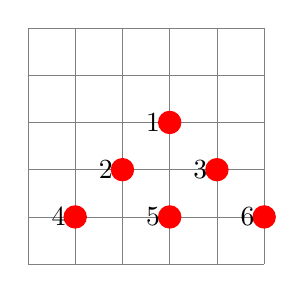
\begin{tikzpicture}[scale=0.60]
			\draw[help lines] (2,2) grid (7,7);

			% circles on l
			\draw [red, fill, ultra thick] (5,5) circle [radius=0.2];
			\draw [red, fill, ultra thick] (4,4) circle [radius=0.2];
			\draw [red, fill, ultra thick] (6,4) circle [radius=0.2];
			\draw [red, fill, ultra thick] (3,3) circle [radius=0.2];
			\draw [red, fill, ultra thick] (5,3) circle [radius=0.2];
			\draw [red, fill, ultra thick] (7,3) circle [radius=0.2];

			% node labels
			\node[left] at (5,5) {$1$} ;
			\node[left] at (4,4) {$2$} ;
			\node[left] at (6,4) {$3$} ;
			\node[left] at (3,3) {$4$} ;
			\node[left] at (5,3) {$5$} ;
			\node[left] at (7,3) {$6$} ;
		\end{tikzpicture}
		\caption{Target Pattern}
		\end{subfigure}
		\begin{subfigure}{0.5\textwidth}
		\label{ccfig2}
		\centering
		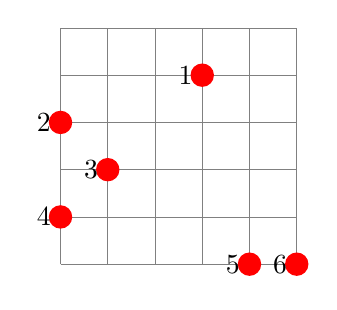
\begin{tikzpicture}[scale=0.60]
			\draw[help lines] (2,2) grid (7,7);

			% circles 
			\draw [red, fill, ultra thick] (2,5) circle [radius=0.2];
			\draw [red, fill, ultra thick] (3,4) circle [radius=0.2];
			\draw [red, fill, ultra thick] (6,2) circle [radius=0.2];
			\draw [red, fill, ultra thick] (2,3) circle [radius=0.2];
			\draw [red, fill, ultra thick] (5,6) circle [radius=0.2];
			\draw [red, fill, ultra thick] (7,2) circle [radius=0.2];

			% node labels
			\node[left] at (2,5) {$2$} ;
			\node[left] at (3,4) {$3$} ;
			\node[left] at (6,2) {$5$} ;
			\node[left] at (2,3) {$4$} ;
			\node[left] at (5,6) {$1$} ;
			\node[left] at (7,2) {$6$} ;
		\end{tikzpicture}
			\caption{Ordering} \label{fig:hi}
		\end{subfigure}
		\caption{Consistent Compass ordering}
	\end{figure}

	Even though consistent compass trivializes APF, the same cannot be said about OneAxis. There are, however,
	two very interesting results also due to Flocchini et. al. which are particularly relevant to our work.
	In particular it's known that:
	\begin{theorem} 
		In a deterministic setting with a \textit{OneAxis} assumption, 
		Arbitrary Pattern Formation is solvable only if $n$ is odd. This is true even in 
		an asynchronous setting.\cite{flocchini08arbitrary}
	\end{theorem} 

	\begin{proof}
		The OneAxis assumption requires that all $n$ robots have consensus on the orientation of one axis. 
		Without loss of generality, we assume the $y$ axis is agreed upon by all robots. Because all robots
		agree on the orientation of the $y$ axis, they can agree on the location of vertical axes $v_1$, 
		$v_2$ which go through the left-most and right-most robots on the plane. In \ref{oddfig1}, for example,
		$r_1$ and $r_3$ are the left-most and right-most robots with such axes going through their positions.
		Note that because we do not have consensus on the direction of the $x$ axis, an arbitrary pair of robots
		$r_i$ and $r_j$ may have a different notion of which among $r_1$ and $r_3$ is the left-most and which is
		the right-most robot. Regardless, the location of $v_1$ and $v_2$ will be the same for all robots.
		As such, in finite time, we can have every robot line up on either $v_1$ or $v_2$, whichever
		axis is closest. Because $n$ is odd, once every robot is on one of the vertical axes, it must
		be that one of the axes has a majority of robots on it. We elect the topmost robot
		on this axis as the leader. As we've shown leader election is enougn to solve the APF problem.
		Figure \ref{oddfig2} gives an example, where the circled robot $r_5$ has been elected leader.

		% TODO: make sure robot notation is consistent r_i

	\end{proof}

	\begin{figure}[H]
		\begin{subfigure}{0.5\textwidth}
		\label{oddfig1}
		\centering
		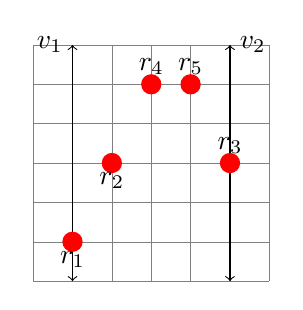
\begin{tikzpicture}[scale=0.50]
			\draw[help lines] (0,0) grid (6,6);

			\draw [<->] (1,0) -- (1,6) ;
			\draw [<->] (5,0) -- (5,6) ;
			% circles
			\draw [red, fill, ultra thick] (1,1) circle [radius=0.2];;
			\draw [red, fill, ultra thick] (2,3) circle [radius=0.2];;
			\draw [red, fill, ultra thick] (5,3) circle [radius=0.2];;
			\draw [red, fill, ultra thick] (3,5) circle [radius=0.2];;
			\draw [red, fill, ultra thick] (4,5) circle [radius=0.2];;

			% node labels
			\node[below] at (1,1) {$r_1$} ;
			\node[below] at (2,3) {$r_2$} ;
			\node[above] at (5,3) {$r_3$} ;
			\node[above] at (3,5) {$r_4$} ;
			\node[above] at (4,5) {$r_5$} ;
			% line labels
			\node[left] at (1,6) {$v_1$} ;
			\node[right] at (5,6) {$v_2$} ;
		\end{tikzpicture}
		\caption{vertical axes}
		\end{subfigure}
		\begin{subfigure}{0.5\textwidth}
		\label{oddfig2}
		\centering
		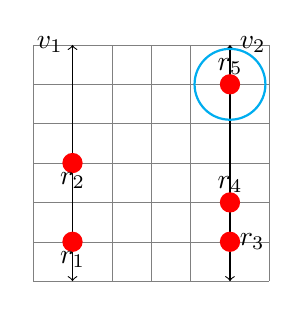
\begin{tikzpicture}[scale=0.50]
			\draw[help lines] (0,0) grid (6,6);
			\draw [<->] (1,0) -- (1,6) ;
			\draw [<->] (5,0) -- (5,6) ;
			% circles
			\draw [red, fill, ultra thick] (1,1) circle [radius=0.2];
			\draw [red, fill, ultra thick] (1,3) circle [radius=0.2];
			\draw [red, fill, ultra thick] (5,1) circle [radius=0.2];
			\draw [red, fill, ultra thick] (5,2) circle [radius=0.2];
			\draw [red, fill, ultra thick] (5,5) circle [radius=0.2];
			\draw [cyan, thick] (5,5) circle [radius=0.9]; % leader circle 
			% node labels
			\node[below] at (1,1) {$r_1$} ;
			\node[below] at (1,3) {$r_2$} ;
			\node[right] at (5,1) {$r_3$} ;
			\node[above] at (5,2) {$r_4$} ;
			\node[above] at (5,5) {$r_5$} ;
			% line labels
			\node[left] at (1,6) {$v_1$} ;
			\node[right] at (5,6) {$v_2$} ;
		\end{tikzpicture}
			\caption{unbalanced configuration} \label{fig:hi}
		\end{subfigure}
		\caption{APF Solved for odd $n$ }
	\end{figure}

\section{Our Results}
\label{ourRes}


In this section we present two distinct approaches to solving APF. The first, which we call PUDDLE, is 
an algorithm that extends a result by Flocchini, et. al. in \cite{flocchini08arbitrary} with randomness.
We produce an algorithm that solves APF for any number of robots, in a disk-based, asynchronous, history
oblivious model with a OneAxis assumption. We further prove that the algorithm is collision-free, and
that it converges on an arbitrary pattern in a bounded number of steps. 
Our second result solves the APF problem again with randomness, but requiring no assumptions on the axes.
Here we use of new method that requires computing the \textit{smallest enclosing circle} (SEC) of
the robot group centered at a common point. We are only able to prove this result for the point-based
model unfortunately.

\subsection{Notation} 
% TODO: necessary??? fix up later, right now just contains ideas
refer to a state $S$ over $n$ robots as $S = (s_1, \ldots s_n)$ where each $s_i \in \RR^2$. For simplicity
$S$ refers to the global view. In refering to the local view of a robot use $S_i$. View is function of orientation
of each bot



$\EE$ is the initial state of all robots, $\PP$ is the final state.

% Armando insert writing here!!!
\subsection{Breaking ties even case } 
	In this section we follow up on a result in \cite{flocchini12distrib} where it's proved that
	APF is solvable deterministically with a OneAxis agreement if the number of robots $n$ is
	odd. Here, we develop a randomized algorithm that solves APF for any number of robots
	and extends the result to the disk-based model. Formally, \cite{flocchini12distrib} states :
	\begin{theorem} 
		Assuming OneAxis, APF is solvable only if $n$ is odd, and this can be done in ASYNC.
	\end{theorem} 

	The result implies that in the a deterministic setting, OneAxis is not a strong enough 
	assumption to solve the APF problem for an even number of robots. Rather than making 
	stronger assumptions about a priori consensus, our result applies randomness to the same setting. 
	We show that this is a strong enough assumption to solve the 
	APF problem with OneAxis in ASYNC. 

	The algorithm we develop proceeds from an initial configuration $\EE$ to produce an input pattern $\PP$.
	Without loss of generality we assume that the $y-axis$ is agreed upon as given by the OneAxis assumption.
	Following the algorithm, robots first attempt to reach consensus on the direction of the x-axis. 
	As shown earlier, this problem is not generally solvable for an even number of robots. In finite time, 
	the robots either reach consensus on the x-axis or elect a leader. The algorithm proceeds as follows
	\begin{enumerate}
		\item Compute two vertical lines $l,r$ tangent to the convex hull of $\EE$, and the vertical line
		at their midpoint $m$. We refer to $L$ as the region on the same side of $l$ with respect to 
		the line $m$, and refer to $R$ similarly .
		\item Let $r$ refer to the line on the side with the majority of robots, and $l$ refer to the side
		with a minority of robots.
		\item If there is a side with a majority of the robots, then we refer to the configuration as
		\textit{unbalanced}, and the side with majority determines the x-axis direction.
		the x axis.
		\item If there is no majority on either side of $m$ (a \textit{balanced } configuration), 
		then with some probability each robot moves to the center line $m$. 
		\item After a finite number of steps, either the robots are all on the same vertical line $m$,
		or they have decided a common direction for the $x$ axis.
		\item If all the robots are on $m$, then we have solved the leader election problem, and 
		can form the arbitrary pattern trivially.
		\item If the configuration is unbalanced, then we apply a different algorithm to order each
		of the robots and form the arbitrary pattern.
	\end{enumerate}

	We note that \cite{flocchini12distrib} provides an algorithm for APF from an unbalanced configuration.
	Since this algorithm assumes a point-based model, we present our own algorithm for this stage of
	the problem. The above algorithm describes the global actions each robot will take. 
	We now give a more detailed view of the algorithm from the viewpoint of the individual robots.
	Due to the length of the algorithm, we present it in sections, and have encapsulated related 
	operations as sub-functions which can be found in the appendix.

	% algorithm
	\begin{algorithm}[H]
	\begin{algorithmic}[1]
	\Procedure{Puddle}{$\EE_i$, $\PP$}
	\caption{PUDDLE part 1}

		% all robots have moved appropriately
		\Switch{$i$.state}
			\Case{START}
				\If{ not isAligned($\EE_i$)} % insert snippet to move onto line l/r
					\State (status, dir) = topmostLR($\EE_i$, i)
					\If{status}
						\State let $h_i$ be the horizontal line through $y_i$
						\State let $l'$ be the vertical axis either $l$ or $r$ in the direction of dir
						\If{ if the point at the intersection of $h_i$ and $l'$ cannot be occupied}
							\State move one unit in the positive $y$ direction.
						\EndIf
						\State move in direction $dir$ along $h_i$ until you are on $l$ or $r$
					\EndIf
				\Else
					\State dest = null
				\EndIf
				\If{ not $\exists$ robot $p$ not on $l$ or $r$}
					\State state = UNBALANCE
				\EndIf
			\EndCase
	\EndProcedure
	\end{algorithmic}
	\end{algorithm}

	\begin{algorithm}[H]
	\begin{algorithmic}[1]
	\caption{PUDDLE part 2: unbalancing}
	\Procedure{Puddle}{$\EE_i$, $\PP$}
		
			\State
			\Case{UNBALANCE}
				\If{ $\exists p \in \EE_i$ not on $l, r,$ or $m$ } \Comment another robot is moving
					\State dest := null
					\State return
				\EndIf
				\If{$|L| = |R|$}
					\State getUnbalanaced()
				\ElsIf{all robots on $m$}
					\State state = ON-M
					\State dest = null
				\Else
					\State state = FORMPATTERN
					\State dest = null
				\EndIf
			\EndCase

			\Case{MOVE\_TO\_M}
				\Comment robot is moving to $m$
					\State let $l'$ be the line from which $i$ originated (either $l$ or $r$), and $L'$ the corresp. side
					\While{ $\exists$ some robot $k$, also on side $L'$ with $y_k < y_i$ }
						\State Wait until robot $k$ is on $m$.
					\EndWhile

					\State Move downward vertically until finding a point $p = (x_p, y_p)$ on $m$ such that 
						moving to $p$ won't block the line of sight of any robot on $l$ or $r$.
					\While{ $\exists$ robot $k$, also moving toward $p$}
						\State with $\frac{1}{2}$ probability keep moving downward
					\EndWhile
						\State dest = $p$
						\State $i$.state = UNBALANCE
			\EndCase
			\State
	\EndProcedure
	\end{algorithmic}
	\end{algorithm}

	\clearpage % avoid having our algorithm moved to the end

	\begin{algorithm}[H]
	\begin{algorithmic}
	\Procedure{PUDDLE}{args}
		\caption{PUDDLE part 3: pattern formation}

			\State
			\Case{FORMPATTERN}
				\State lineup()
				\State formPattern()
			\EndCase

			\State
			\Case{ON-M}
				\State leaderPattern()
			\EndCase

			\State
			\Case{DONE}
				\State // do nothing the algorithm has finished
			\EndCase
		\EndSwitch

	\EndProcedure
	\end{algorithmic}
	\end{algorithm}
	
	We must now prove that the algorithm above is both collision free and coverges to a solution
	that correctly solves APF.
	\subsection{PUDDLE runs in linear time} 
		We break up our analysis into three parts, each of which will be in linear time. The algorithm
		begins in the START state, which arranges all robots on a the vertical tangents to the convex
		hull $l$ and $r$. Each robot $i$ moves according to the topmost() function in the appendix, which requires
		that robot $i$ be the topmost robot according to $y$ coordinate. Consequently, in the worst case 
		the robots move one	at a time onto lines $l$ and $r$. Thus, $O(n)$ move steps are required to 
		complete this stage of the algorithm; where $n$ is the number of robots.
		% TODO ensure the robots initially on $l$ and $r$ move downward for the above to work

		Now we examine the unbalance procedure. Fix an arbitrary iteration of the unbalance procedure with,
		there are exactly $\frac{k}{2}$ robots on $l$ and on $r$ each, and $n - k$ robots on line $m$. 
		Thus, for any robot $i$ on $l$ or $r$ the probability that robot $i$ moves is 
		$Pr(i \text{ moves }) = \frac{1}{k}$. The unbalance procedure will fail to create an unbalanced configuration
		only if no robots move to $m$ on this iteration or the same number of robots from each side move
		in this iteration. % define notion of an iteration more precisely
		The probability that no robots move is given by $(1 - \frac{1}{k})^{k} \leq \frac{1}{e}$. 
		The probability that $i$ robots from a single side move to $m$ in the same iteration is given 
		by the binomial distribution: $(\frac{1}{k})^i (\frac{k-1}{k})^{k-i} {k\choose i}$.
		The probability that the same number of robots move from each side in an iteration is given 
		by a sum of squares over the binomial distribution:
		$$\sum_{i=1}^{k}{((\frac{1}{k})^i (\frac{k-1}{k})^{k-i} {k\choose i})^2} \label{eq1}$$

		\ref{eq1} is $\leq  .20 \text{ for } 
		%\ref{eq1} is equal to $((\frac{k-1}{k})^{2k} ) \cdot ( F_1(-k, -k ; 1 ; \frac{1}{(k-1)^2}) - 1) \leq .20 \text{ for } 
		k \geq 6$. Since, $\frac{1}{e} \leq .37$, the total probability of failure is $\leq .57$. Considering, a complete
		iteration as a Bernoulli process with success probability $p = 0.43$, the expected number of iterations until 
		an unbalanced configuration is reached is $\frac{1}{p} \approx 2.32$. Thus, we expect a constant number of iterations
		as $n$ grows asymptotically. To bound the amount of work done in a single iteration, we consider the worst case
		where all robots on both $l$ and $r$ decide to move, and must reach consensus on placement in line $m$. 
		The relevant code is in the MOVE\_TO\_M case of the PUDDLE algorithm. On each side, the algorithm requires that only 
		one robot be moving vertically to locate a position on line $m$. Consensus, reduces to the case where a robot
		from $q_l$ and a robot from $q_r$ from $l$ and $r$ respectively both attempt to enter 
		points $p_l$ and $p_r$ on $m$ that are within unit distance. At this point, we again use randomness
		to break ties. Ideally, we would like one of $q_r$ or $q_l$ to continue looking for the next available point,
		and the other to take its intended point. This happens with probability $\frac{1}{2}$. Otherwise, the robots 
		continue to block each other from entering $m$. It's easy to see that in expectation two attempts to reach
		consensus are necessary before the robots are both able to enter $m$. Thus, in the worst case we must deal with
		$O(n)$ conflicts in a single iteration of the unbalance procedure. These conflicts can be resolved in 
		constant time so at worst $O(n)$ work is required per iteration. Since a constant number of iterations are 
		required, we've shown the second stage of the algorithm to run in a linear number of steps. \\

		The final stage of PUDDLE is running either the formPattern() or the leaderPattern() routines depending on
		whether consensus on an x-axis is reached or all robots end up on line $m$. In both cases we first run the 
		uniformSpacing() procedure to ensure that the distance between robots on the same vertical axis is uniform.
		This procedure takes $O(n)$ steps since each robot moves only after one of it's neighbors has, and in 
		the worst case, the robots move one at a time. formPattern() then has each robot compute its relative
		distance to the top-most robot to establish a total ordering of the robots. This step
		, done by each robot, requires $O(n)$ computations. The total ordering is then used to assign a
		unique point each robot must assume in the target pattern $\PP$, and the robots move to these 
		assigned points serially requiring $O(n)$ steps to do this. The leaderPattern() function behaves almost
		identically, except for an additional step, where we require the leader to move $n-1$ units along the
		$x$ axis to help establish a total ordering. \\

		All of the steps described tell us that our algorithm will run in a number of steps linear in the 
		number of robots.  

		% TODO: mention that both size and orientation are preserved unlike previous algorithm

		\subsection{PUDDLE is collision free} 
		As in the previous section, we consider the algorithm in three separate parts. During the START phase
		we can be assured that arranging the $n$ robots on $l$ and $r$ will be collision-free because only the
		robot with the largest $y$-coordinate (called $y_{max}$) will move. In the case of ties, only the two robots
		on the horizontal line through $y_{max}$ with the smallest and largest $x$-coordinates will move, and toward
		vertical line $l'$ as given by the algorithm to prevent collisions. 
		If a position on $l'$ is already occupied, a robot $i$
		moves in the positive $y$ direction. Since, $i$ was already the top-most robot not on $l$ or $r$, no collision
		can occur in this move. \\

		In the unbalance stage of the algorithm, we note that all robots on a given side $L'$ move vertically at a point 
		that is a unique distance from $l'$. Furthermore only the robot with the smallest $y$ coordinate
		moves to enter the middle line $m$. Thus, collisions cannot occur between robots of on the same side $L'$.
		To avoid collisions between a robot moving from $l$ and another moving from $r$ into line $m$, we ensure each
		robot $i$ only enter $m$ on point $p_i$ if there is no other robot $j$ moving toward a point $p_j$ on $m$
		that is within unit distance of $p_i$. If there is such a robot, $i$ stops, and only moves toward $p_i$ if
		robot $j$ has moved vertically, away from point $p_j$, or if $i$ decides to move vertically to find a 
		different entry point into $m$. Hence, collisions between robots from $l$ and $r$ are avoided as well. \\

		In the formPattern() and leaderPattern() stages, we avoid collisions by having only a single robot move to
		it's target position in pattern $\PP$ at any given time. The points in $\PP$ are sequenced by 
		decreasing $y$ coordinate, and decreasing $x$ coordinate. Thus, when robot $i$ moves to point $\PP_i$ in 
		the final configuration, none of the robots already in the configuration will get in the way of $i$. \\

		% TODO: move robots back from m to $l$ or $r$

		\subsection{additional properties of algorithm} 
		Our algorithm also observes some additional properties that the original algorithm by Flocchini did not.
		Firstly, our algorithm not only produces the given input pattern without rotation, but unlike \cite{flocchini12distrib},
		the original pattern's dimensions are preserved. There is no rescaling.




		


	



% goals for this section
% describe section
% give high level desc of result
% give detailed desc with algorithm etc
%
% insert descriptions of graphics needed (if any)
% flesh out algorithm in sufficient detail
% add stuff to appendix if necessary
% follow similar style as previous papers
% conclude with 

% Siva insert writing here!!!
\subsection{SEC stuff } 

\section{Conclusion}
\label{conc}

%% The Appendices part is started with the command \appendix;
%% appendix sections are then done as normal sections
%% \appendix

%% \section{}
%% \label{}
\appendix
\section{Helper Procedures for PUDDLE}
\subsection{topmostLR()} 

% TODO define robots not on $l, r$: 
% We refer to robots that aren't on the $l$ or $r$ to be unaligned
Let $y_max$ be the largest y-coordinate of any unaligned robot. 
This method returns true if robot $i$ is the topmost unaligned robot by $y$ coordinate. In the
case of ties, the method returns true only if $i$ is the left-most or right-most 
robot on the horizontal line through $y_{max}$.

\begin{algorithm}[H]
\begin{algorithmic}[1]
\Procedure{topmostLR}{$\EE_i$, $i$}
	\State $E'_i = \{ (x_j, y_j) \in E_i : \text{ robot j isn't on line } r \text{ or } l\}$
	\State $y_{max} = \max_{(x_j, y_j) \in E'_i}{y_j}$ 
	\State $x_{max} = \max_{(x_j, y_j) \in E'_i : y_j = y_{max} }{x_j}$ 
	\State $x_{min} = \min_{(x_j, y_j) \in E'_i : y_j = y_{max} }{x_j}$ 

	\If{ $(x_i, y_i) == (x_{max}, y_{max})$ }
		\State return $(True, right)$
	\ElsIf{ $(x_i, y_i) == (x_{max}, y_{max})$ }
		\State return $(True, left)$
	\Else
		\State return $(False, null)$
	\EndIf

\EndProcedure
\end{algorithmic}
\end{algorithm}

\subsection{isAligned()} 

This method computes the convex hull vertical tangent lines $l$ and $r$ according
to the local view of robot $i$. We return true if $i$ is on one of the 
computed tangents.
\begin{algorithm}[H]
\begin{algorithmic}[1]
\Procedure{isAligned}{$\EE_i$}
	\State compute $l,r$ from local view $\EE_i$
	\If $(x_i, y_i) \notin  l$ and $(x_i, y_i) \notin r$
		\State return False
	\Else 
		\State return True
	\EndIf
\EndProcedure
\end{algorithmic}
\end{algorithm}

\subsection{getUnbalanced()} 
Here we apply randomness to have a robot move from either $l$ or $r$ to $m$.
This helper module gives our algorithm the additional power necessary to 
solve APF in the even case.
\begin{algorithm}[H]
\begin{algorithmic}[1]
\Procedure{getUnbalanced}{$\EE_i$}
	\If{ $i$ is on $m$ already}
		\State dest = null
		\State return
	\EndIf
	\State compute $m$ from local view
	\State compute $b$ from local view of $m$ and $t$
	\State move = True with probability $\frac{1}{b}$ \Comment move horizontally to line $m$. 
	\If{ move}
		\State state = MOVE\_TO\_M
		% TODO: notion of doppleganger or something for bot directly across from you
		\State let $l'$ refer to the vertical tangent (either $l'$ or $r'$) that $i$ is on
		\State compute rank = numeric ordering of $i$ counting from top to bottom on $i$
		\State let $h_i$ be the horizontal line through $y_i$. 
		\State compute point $p$ which is $rank$ units toward $m$ on line $h_i$.
		\State dest = $p$
	\EndIf


	% TODO: be precise about how robots align selves on $m$
\EndProcedure
\end{algorithmic}
\end{algorithm}

%\subsection{avoidCollision} 

\subsection{lineup()} 
	\begin{algorithm}[H]
	\begin{algorithmic}[1]
	\Procedure{lineup}{$\EE_i$, $\PP$}
		
		\Comment ensure that top-most guys line up
		\State Let $t_l$ and $t_r$ refer to the top-most robots on $l$ and $r$
		\If{ $i$ is  $t_l$ and $y_{t_l} > y_{t_r}$}
			\State set dest = $(x_i, y_{t_r})$
		\ElsIf{ $i$ is  $t_r$ and $y_{t_r} > y_{t_l}$}
			\State set dest = $(x_i, y_{t_l})$
		\Else 
			\State dest = null
		\EndIf

		\State uniformSpacing()
	\EndProcedure
	\end{algorithmic}
	\end{algorithm}

\subsection{formPattern()} 
	\begin{algorithm}[H]
	\begin{algorithmic}[1]
	\Procedure{formPattern}{$\EE_i$, $\PP$}

		\If{$i$ is top-most robot on $l$} % distinguish between $l$ after x-axis consensus and global $x$ explain
			\State let $h$ = height of target pattern $\PP$.
			\State dest = $(x_i + 1, y_i + h)$
		\EndIf
		\While{ top robot on $l$ is not at $(x_i + 1, y_i + h)$}
			Wait
		\EndWhile

		\State Use distance to top-most robot in other vertical line to compute your 
		ordering number $n_i$
		\State dest = $N(\PP)[n_i]$
		\While{there is a robot above you}
			Wait
		\EndWhile
		\State move to dest
		state = DONE

	\EndProcedure
	\end{algorithmic}
	\end{algorithm}
\subsection{formPattern()} 
This method is called to finish forming the pattern in the case where
a common $x$ axis is determined.
\begin{algorithm}[H]
\begin{algorithmic}[1]
\Procedure{formPattern}{$\EE_i$, $\PP$, dir}
	\Switch{state}
		\Case{LEFT}
			
		\EndCase
	\EndSwitch
\EndProcedure
\end{algorithmic}
\end{algorithm}

\subsection{uniformSpacing()} 
This is a utility algorithm that establishes a uniform spacing between all robots on
the same vertical line.
\begin{algorithm}[H]
\begin{algorithmic}[1]
\Procedure{uniformSpacing}{$\EE_i$}
	\If{$i$ is the top-most robot on $m$}
		\State move up two units
	\EndIf
	\State let $j$ be the robot immediately above $i$ on $m$.
	\State compute point $p$ on $m$ such that $j$ is one
	unit above $i$ on $m$.
	\State move to $p$.

	% how ensure we're done moving??
	% once done move one unit L or R, first bot decides direction
	\While{ $\exists$ robot $p$ still moving along $m$ }
		\State wait
	\EndWhile
\EndProcedure
\end{algorithmic}
\end{algorithm}

\subsection{leaderPattern()} 
This method is called to form a pattern when all robots are on $m$.
\begin{algorithm}[H]
\begin{algorithmic}[1]
\Procedure{leaderPattern()}{$\EE_i, \PP$}

	uniformSpacing($\EE_i$) % TODO: add state, so we know we've done this once
	\If{$i$ is the top-most robot}
		\State compute point $p$, right $(n-1)$ units from $i$'s current location
		\State dest = p
	\Else
		dest = null
	\EndIf

	\While{ top-most robot is still moving }
		\State wait
	\EndWhile

	\State Use distance to top-most robot to compute position $p$ that you
	should assume in the final configuration.

	\While{ $\exists$ robot $j$ above you on $m$}
		\State wait
	\EndWhile
	\State dest = $p$
	\State state = DONE


	% TODO: setup an artifical ordering notation on the points in the shape!!
\EndProcedure
\end{algorithmic}
\end{algorithm}
%% If you have bibdatabase file and want bibtex to generate the
%% bibitems, please use
%%
%%  \bibliographystyle{elsarticle-num} 
%%  \bibliography{<your bibdatabase>}

\bibliographystyle{elsarticle-num} 
\bibliography{report}

\end{document}
\endinput

% TODO
%
% intro
% previous results
% my algorithm
% Siva's stuff
% conclusion

%HAVE SIVA LOOK AT
% abstract -- reuse Siva's

